%%%%%%%%%%%%%%%%%%%%%%%%%%%%%%%%%%%%%%%%%%%%%%%%%%%%%%%%%%%%%%%%%%%%%%%%%%%%%%%%
% SD Lab -- Topic
% Giovanni Ciatto
% Alma Mater Studiorum - Università di Bologna
% mailto:giovanni.ciatto@unibo.it
%%%%%%%%%%%%%%%%%%%%%%%%%%%%%%%%%%%%%%%%%%%%%%%%%%%%%%%%%%%%%%%%%%%%%%%%%%%%%%%%
%\documentclass[handout]{beamer}\mode<handout>{\usetheme{default}}
%
\documentclass[presentation]{beamer}\mode<presentation>{\usetheme{AMSBolognaFC}}
%\documentclass[handout]{beamer}\mode<handout>{\usetheme{AMSBolognaFC}}
%%%%%%%%%%%%%%%%%%%%%%%%%%%%%%%%%%%%%%%%%%%%%%%%%%%%%%%%%%%%%%%%%%%%%%%%%%%%%%%%
\usepackage{sd-lab-common}
\usepackage{sd-lab-consensus}
%%%%%%%%%%%%%%%%%%%%%%%%%%%%%%%%%%%%%%%%%%%%%%%%%%%%%%%%%%%%%%%%%%%%%%%%%%%%%%%%
\title[\currentLab{} -- Consensus]{
	Consensus
}
%
\subtitle{\courseName{} (\courseAcronym) / Module \moduleN{}}
%
\author[\sspeaker{\mmShort} \& \gcShort]{
	\speaker{\mmFull} \and \gcFull
	\\ 
	\mmEmail \and \gcEmail
}
%
\institute[\disiShort, \uniboShort]{\disi{} (\disiShort)\\\unibo}
%
\date[A.Y. \academicYear{}]{Academic Year \academicYear{}}
%
%%%%%%%%%%%%%%%%%%%%%%%%%%%%%%%%%%%%%%%%%%%%%%%%%%%%%%%%%%%%%%%%%%%%%%%%%%%%%%%%
\begin{document}
%%%%%%%%%%%%%%%%%%%%%%%%%%%%%%%%%%%%%%%%%%%%%%%%%%%%%%%%%%%%%%%%%%%%%%%%%%%%%%%%

%/////////
\frame{\titlepage}
%/////////

%%===============================================================================
\section*{Outline}
%%===============================================================================
%
%%/////////
\frame[c]{\tableofcontents[hideallsubsections]}
%%/////////

%===============================================================================
\section{Motivation and Goals}
%===============================================================================

\begin{frame}{Lecture Goals}
	\begin{itemize}
		\item 
	\end{itemize}
\end{frame}

\begin{frame}{Motivations}
	\begin{itemize}
		\item 
	\end{itemize}
\end{frame}

%===============================================================================
\section{Assumptions}
%===============================================================================

\begin{frame}{Time}
	\begin{itemize}
		\item (Full) synchrony $\rightarrow$ each message between correct nodes is delivered within a time interval $\Delta$;
        %
        \item Eventual synchrony $\rightarrow$ the system becomes (full) synchronous after one unknown point in time (Global Stabilisation Time);
        %
        \item Partial synchrony $\rightarrow$ the system is synchronous but $\Delta$ is unknown;
        %
        \item Weak synchrony $\rightarrow$ $\Delta$ can increase over time $t$ (at most polynomially);
        %
        \item Asynchrony $\rightarrow$ no time assumption on message delivery, i.e. eventually a message will be delivered.
	\end{itemize}
\end{frame}

\begin{frame}{Faults}
    In the real world things are far from ideals.
    %
    There could be faults of any sort for any reason.
    %
    When designing a consensus algorithm one should consider:
    %
    \begin{itemize}
        \item Crash fault $\rightarrow$ a node stop working or its messages are not delivered;
        %
        \item Byzantine fault $\rightarrow$ a node start behaving unpredictably (it can also be malicious).
    \end{itemize}
\end{frame}

%===============================================================================
\section{Raft}
%===============================================================================

\begin{frame}{Properties}
    \begin{itemize}
        \item Easy to understand $\rightarrow$ authors have deliberately chosen to prioritise understandability (Occam's razor);
        %
        \item Safety or correctness $\rightarrow$ if any server has applied a particular log entry to its state machine, then no other server may apply a different command for the same log index;
        %
        \item Asymmetric or leader-base $\rightarrow$ strong leader, log entries only flow from the leader to the other serves;
        %
        \item Crash fault tolerance $\rightarrow$ $N \ge 2F + 1$ therefore $F \le \frac{N - 1}{2}$;
        %
        \item Membership changes $\rightarrow$ the system can continue to operate during changing in the set of servers.
    \end{itemize}
\end{frame}

\begin{frame}[allowframebreaks]{Model}
    
    \begin{block}{In a nutshell}
        First of all, RAFT servers start electing one leader.
        %
        The leader accepts client's requests and replicates them to the other servers.
        %
        If the leader crashes, a new election starts and eventually a new leader is elected.
    \end{block}
    
    \framebreak
    
    There are three possible states for a node:
    \begin{itemize}
        \item Leader  $\rightarrow$ handles all client requests;
        %
        \item Follower $\rightarrow$ responds to requests from leader and candidates;
        %
        \item Candidate $\rightarrow$ tries to be elected in the leader election phase.
    \end{itemize}

    \centering
    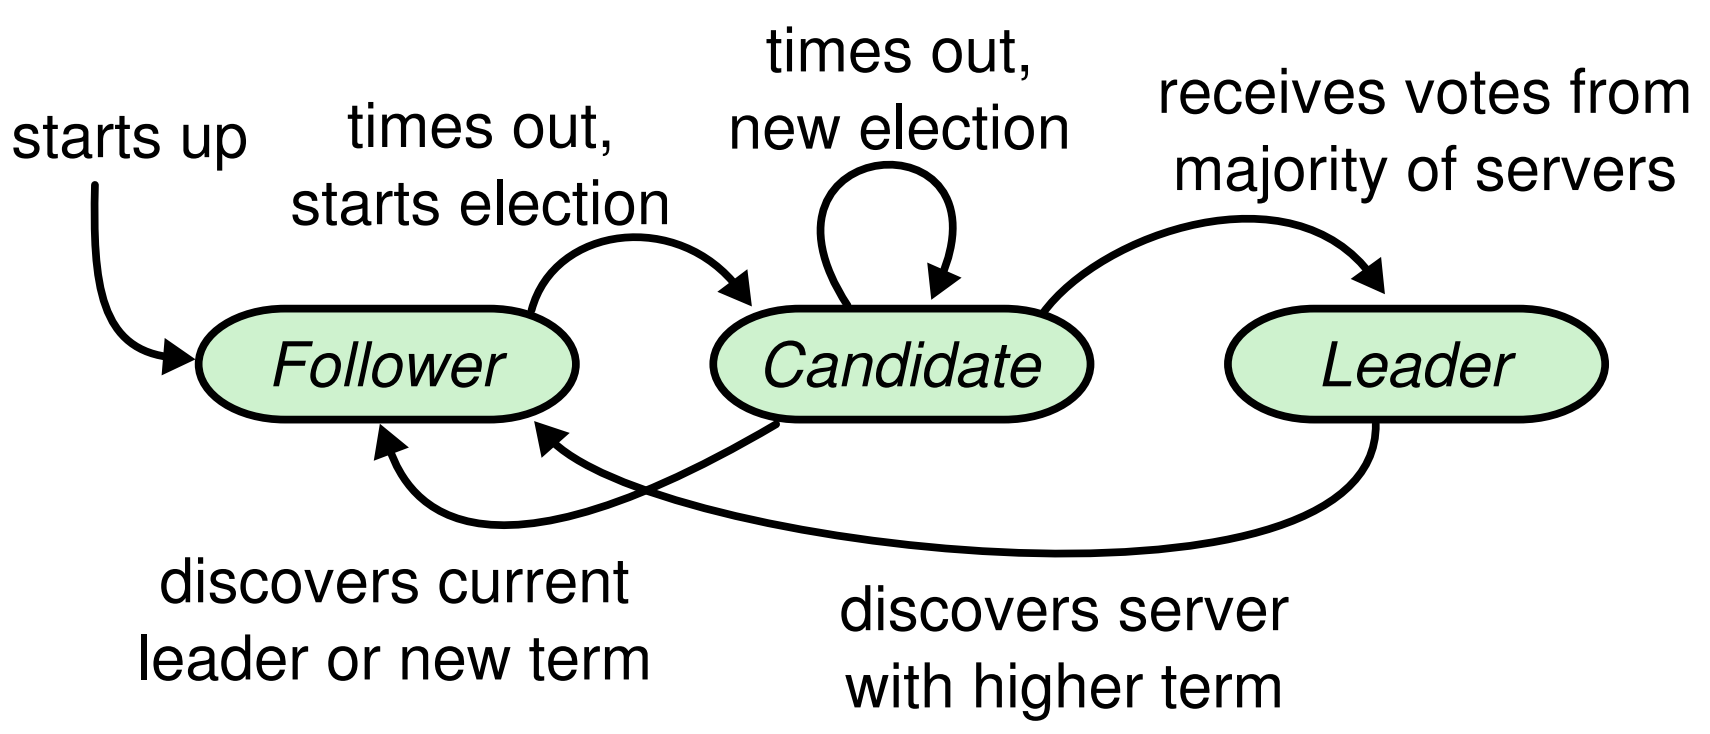
\includegraphics[width=0.8\textwidth]{figures/node-state-diagram.png}
    
    \framebreak
    
     \begin{block}{Time}
        Time is divided into \emph{terms} of arbitrary length.
        %
        Terms are numbered with consecutive integers.
        %
        Each \emph{term} begins with an election.
        %
        If a candidate wins it is the leader for the rest of the \emph{term}.
        %
        If the election results in a split vote the \emph{term} finishes and a new \emph{term} will begin.
    \end{block}

    \centering
    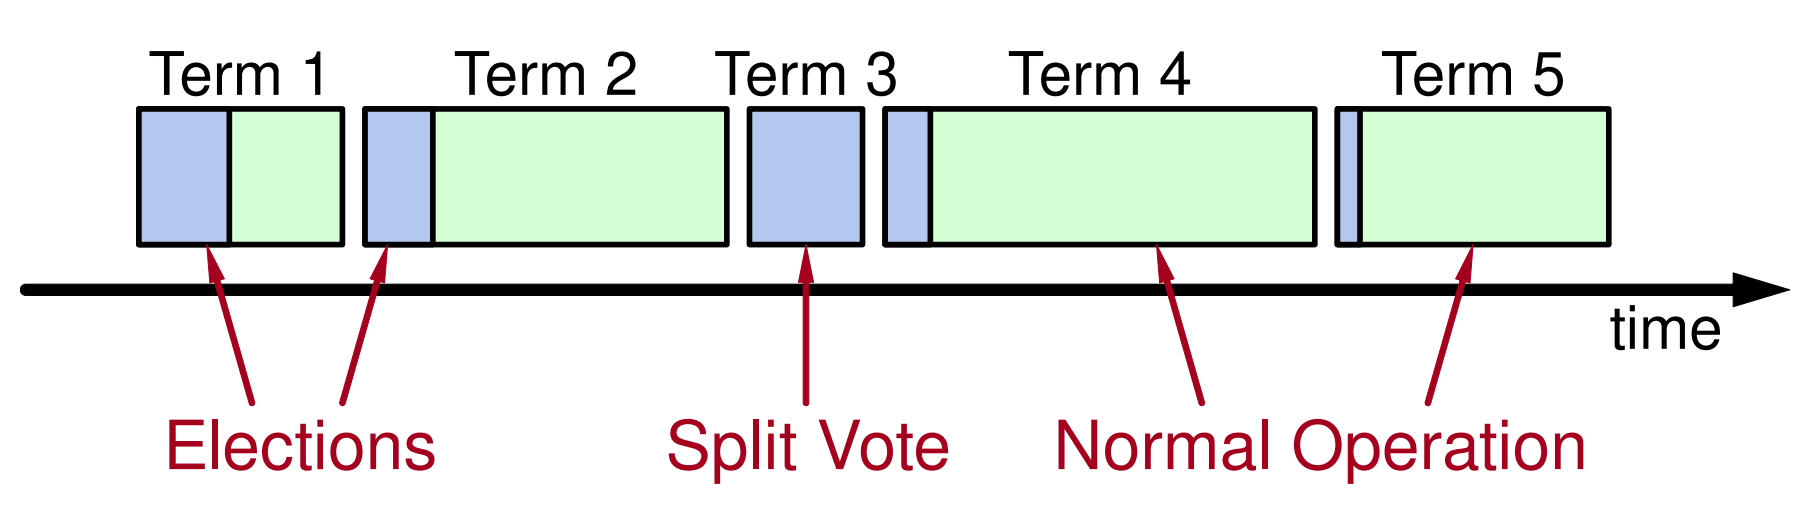
\includegraphics[width=0.8\textwidth]{figures/time.png}
    
    \framebreak
    
    \begin{block}{Leader election}
        Heartbeats are used to trigger leader election.
        %
        When a server starts it begins as \emph{follower}.
        %
        A server remains \emph{follower} as long as it receives a valid heartbeat from a \emph{leader} or \emph{candidate}.
        %
        If a \emph{follower} receives no communication over a period of time, then it assumes there is no available leader and begins an election.
        %
        A \emph{candidate} stays in this state until:
        \begin{itemize}
            \item it wins the election ($\rightarrow$ \emph{leader});
            %
            \item another server wins the election ($\rightarrow$ \emph{follower});
            %
            \item a period of time goes with no winner ($\rightarrow$ new \emph{term});.
        \end{itemize}   
 \end{block}
    
    \framebreak
    
    \begin{block}{Log replication}
        When receiving a command the \emph{leader} appends it to its log as a new entry.
        %
        Then it send the entry to the other servers for replication.
        %
        When the entry has been safely replicated, the \emph{leader} applies the entry to its state machine and returns the result of that execution to the client.
        %
        If \emph{followers} crash or run slowly, or if network packets are lost, the \emph{leader} retries.
    \end{block}

    \framebreak

    \centering
    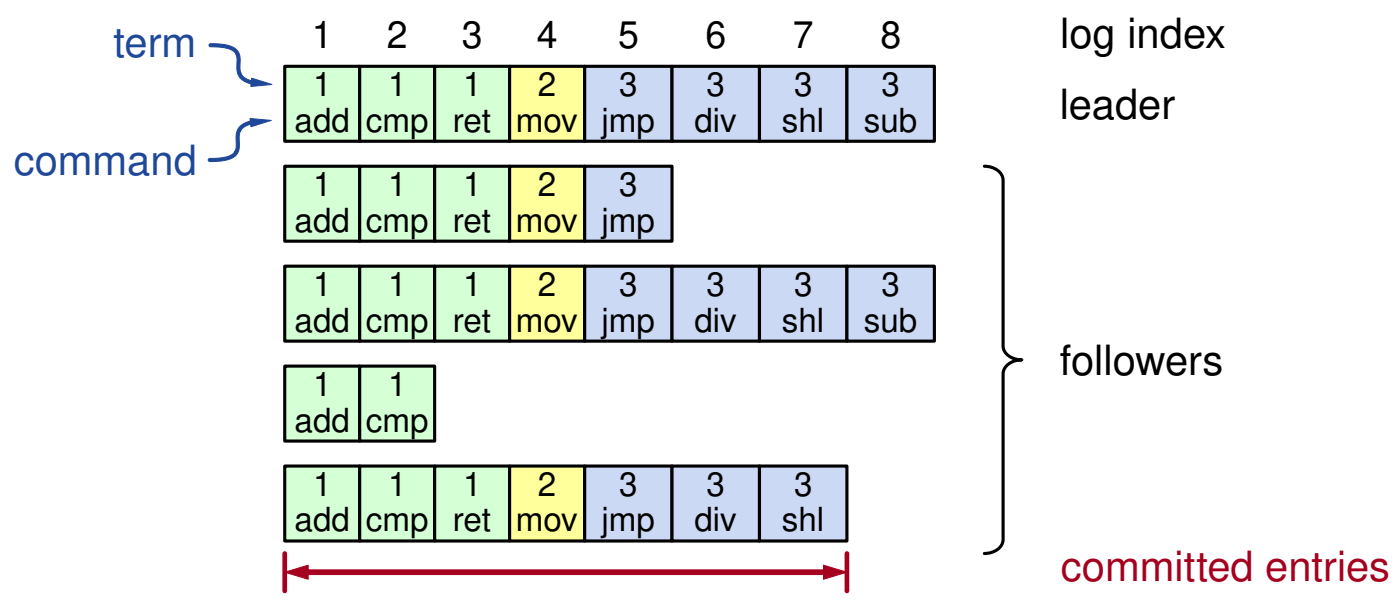
\includegraphics[width=0.8\textwidth]{figures/log.png}

\end{frame}

%===============================================================================
\section{Etcd}
%===============================================================================

\begin{frame}{Etcd}
	\begin{block}{What is etcd?}
		``Etcd is a strongly consistent, distributed key-value store that provides a reliable way to store data that needs to be accessed by a distributed system or cluster of machines.
        %
        It gracefully handles leader elections during network partitions and can tolerate machine failure, even in the leader node.''
        %
        \begin{flushright}
            (\href{https://etcd.io/}{etcd.io})
        \end{flushright}
	\end{block}
	%
\end{frame}

%===============================================================================
\section*{}
%===============================================================================

%/////////
\frame{\titlepage}
%/////////

%===============================================================================
\section*{\refname}
%===============================================================================

%%%%
\setbeamertemplate{page number in head/foot}{}
%/////////
\begin{frame}[c,noframenumbering]{\refname}
%\begin{frame}[t,allowframebreaks,noframenumbering]{\refname}
%	\tiny
	\scriptsize
%	\footnotesize
	\bibliographystyle{apalike-AMS}
	\bibliography{sd-lab-consensus}
\end{frame}
%/////////

%%%%%%%%%%%%%%%%%%%%%%%%%%%%%%%%%%%%%%%%%%%%%%%%%%%%%%%%%%%%%%%%%%%%%%%%%%%%%%%%
\end{document}
%%%%%%%%%%%%%%%%%%%%%%%%%%%%%%%%%%%%%%%%%%%%%%%%%%%%%%%%%%%%%%%%%%%%%%%%%%%%%%%%
